\section{Topological Analysis}

\subsection{Cubical Persistent Homology as a Predictive Ablation}

Cubical persistent homology was evaluated over raw images, morphology-conditioned distance maps, nucleus and cytoplasm candidates, CNN feature-map filtrations, early fusion, and late fusion. These experiments were useful because they tested whether topological summaries add predictive unknown-detection signal beyond deep embeddings. The answer under the evaluated protocol is negative. TDA-only features encode some class information, with the Delivery 2 TDA-only closed macro-F1 reaching 0.828, but open-set AUROC remains approximately 0.55--0.58 for TDA-only variants, and Deep+TDA fusion degrades the principal deep baseline. Delivery 3 morphology-aware and feature-map variants also fail the predeclared progression rule.

This is not a claim that topology contains no biological or morphological information. It is a narrower claim: the evaluated cubical persistent-homology representations did not provide robust complementary unknown-detection utility under the frozen protocol. The detailed ablations belong in the supplement because they support claim discipline without displacing the central external-validation result.

\subsection{Vietoris-Rips Embedding Topology}

The Vietoris-Rips analysis is secondary and explanatory. It comprises 500 cloud analyses over MLL23 and AML-LMU, V1 and V2 training splits, CE and ArcFace representations, five seeds, and known plus predeclared hard unknown morphology clouds. Each cloud has $H_0$ and $H_1$ summaries, producing 1,000 homology summary rows. The construction uses L2-normalized embeddings, cosine distance, $N_{VR}=192$, a fixed sample seed, and GUDHI 3.13.0.

The VR results are mixed. H0 bottleneck summaries are generally larger for ArcFace than CE across seed and split comparisons, but H1 behavior is weaker and not a clean explanation of open-set performance. The topology--OSR correlations are exploratory and inconsistent. The strongest observed associations involve mean known H1 total persistence and ViM metrics, but the broader pattern does not support predictive or causal claims. For MSP AUROC, mean known H1 max persistence has Pearson $r=0.148$ and Spearman $\rho=0.014$, while Fisher ratio has Pearson $r=-0.138$ and Spearman $\rho=0.030$ in the conventional geometry correlation table.

\begin{figure}[htbp]
\centering
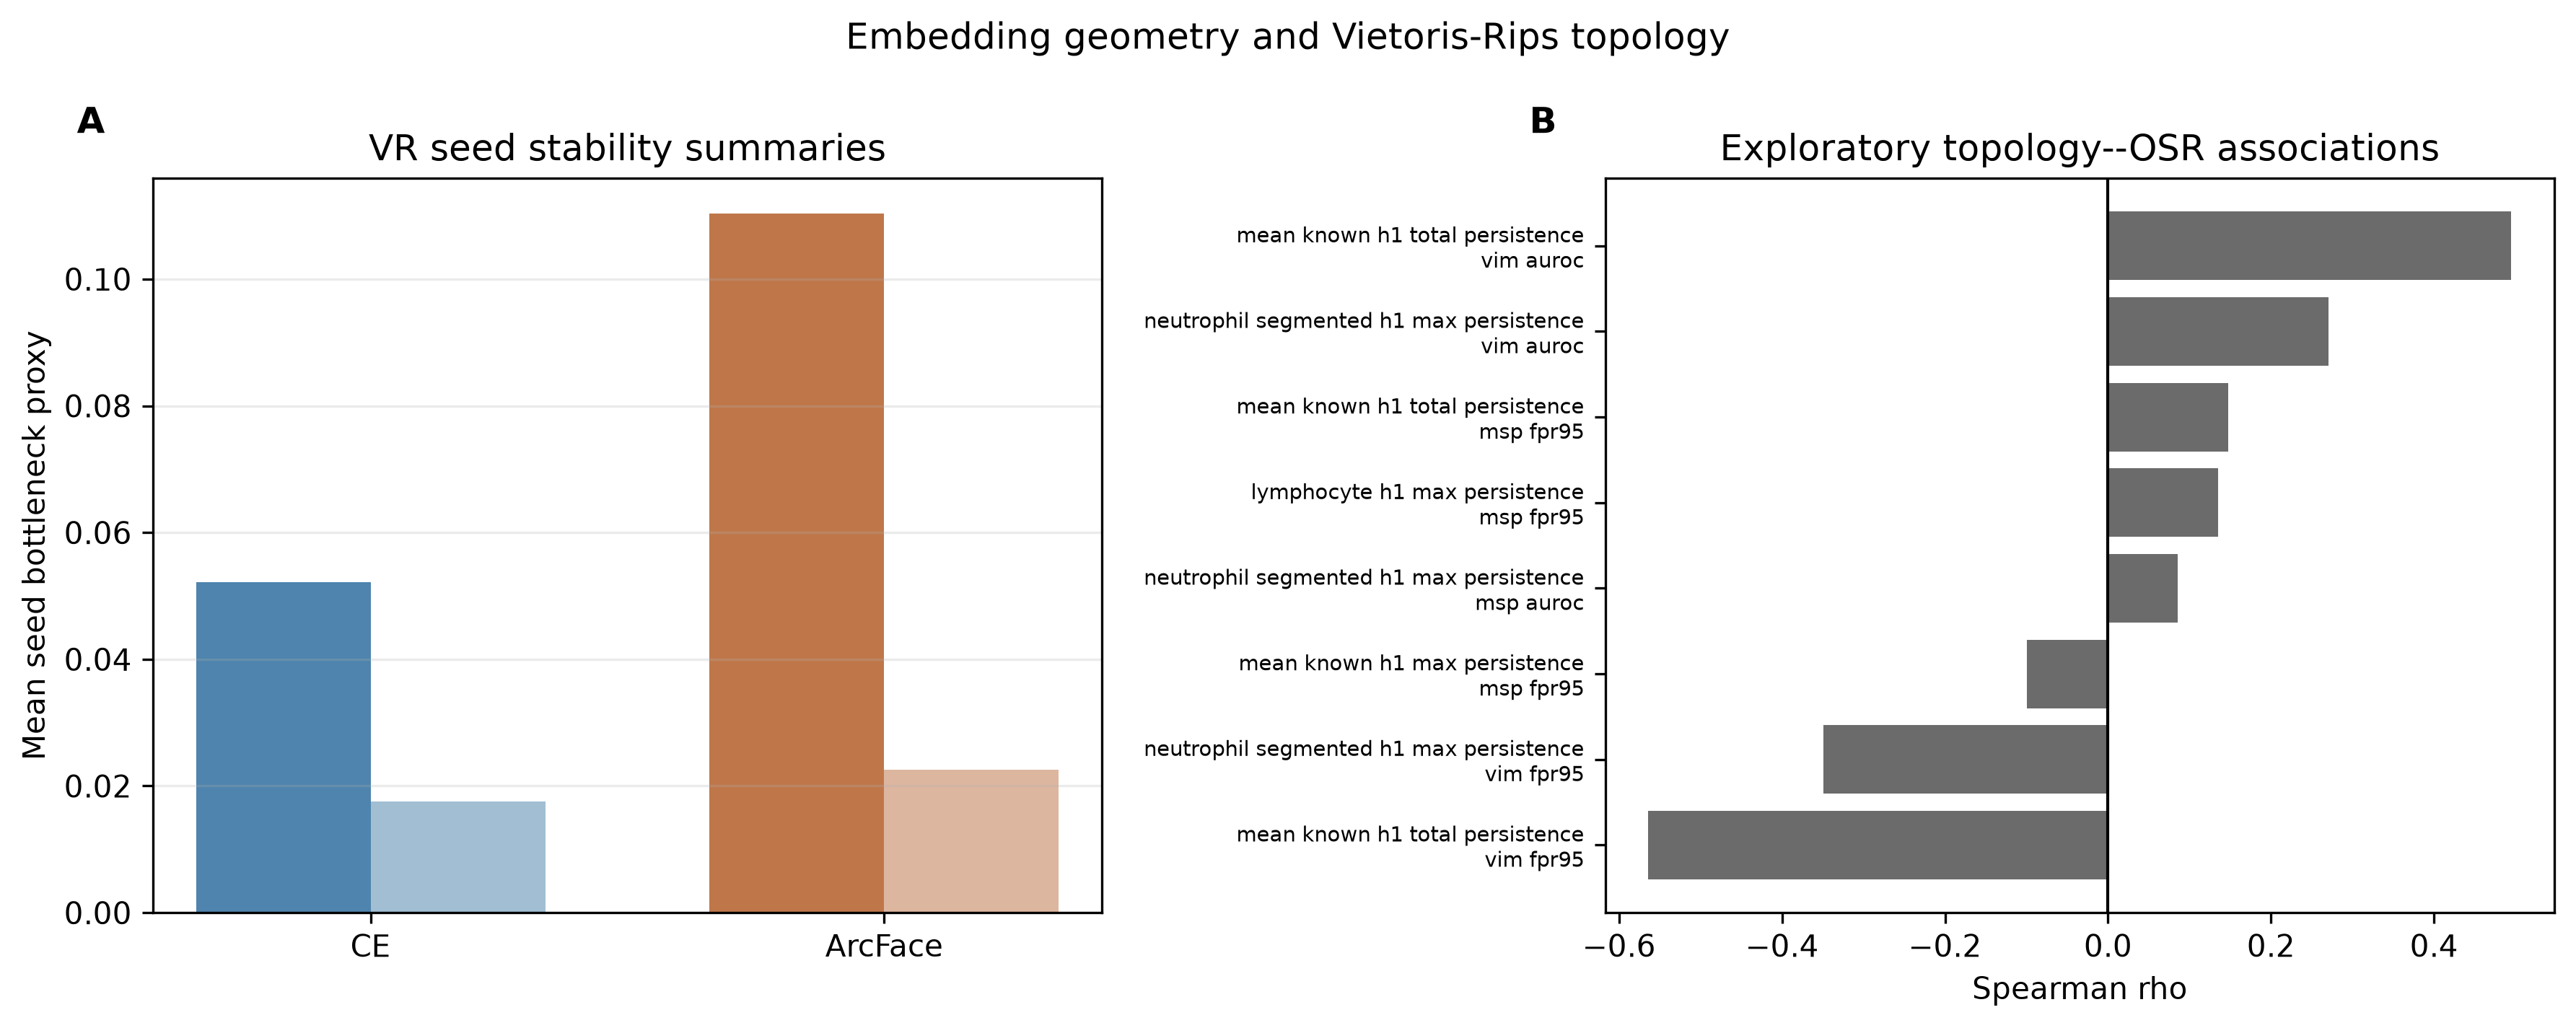
\includegraphics[width=\textwidth]{figures/figure7_topology.png}
\caption{Vietoris-Rips topology summaries and exploratory associations with OSR metrics. The analysis is descriptive only and is not used for prediction.}
\label{fig:topology}
\end{figure}
